%% LyX 2.3.2 created this file.  For more info, see http://www.lyx.org/.
%% Do not edit unless you really know what you are doing.
\documentclass[12pt,english]{article}
\usepackage{ae,aecompl}
\usepackage[T1]{fontenc}
\usepackage[latin9]{inputenc}
\usepackage{geometry}
\geometry{verbose,tmargin=3cm,bmargin=3cm,lmargin=2.5cm,rmargin=2.5cm}
\usepackage{xcolor}
\usepackage{pdfcolmk}
\usepackage{float}
\usepackage{textcomp}
\usepackage{url}
\usepackage{amstext}
\usepackage{amssymb}
\usepackage{graphicx}
\usepackage{setspace}
\usepackage{esint}
\usepackage[authoryear]{natbib}
\PassOptionsToPackage{normalem}{ulem}
\usepackage{ulem}
\doublespacing

\makeatletter

%%%%%%%%%%%%%%%%%%%%%%%%%%%%%% LyX specific LaTeX commands.
\providecolor{lyxadded}{rgb}{0.15,0.55,0.82}
\providecolor{lyxdeleted}{rgb}{0.83,0.21,0.51}
%% Change tracking with ulem
\DeclareRobustCommand{\lyxadded}[3]{{\color{lyxadded}{}#3}}
\DeclareRobustCommand{\lyxdeleted}[3]{{\color{lyxdeleted}\lyxsout{#3}}}
\DeclareRobustCommand{\lyxsout}[1]{\ifx\\#1\else\sout{#1}\fi}

%%%%%%%%%%%%%%%%%%%%%%%%%%%%%% User specified LaTeX commands.
\usepackage{aecompl}\usepackage{lineno}






\usepackage{babel}

\makeatother

\usepackage{babel}
\begin{document}
\title{Looking for compensation at multiple scales in a wetland bird community}
\author{{\Large{}{}Fr�d�ric Barraquand$^{1,2,*}$, Coralie Picoche$^{1}$,
Christelle Aluome$^{1,3}$, }\\
 {\Large{}{}Laure Carassou$^{1,4}$ \& Claude Feign�$^{5}$}}

\maketitle
{\large{}{}\bigskip{}
}{\large\par}

{\large{}{}}\textsuperscript{{\large{}{}1}}{\large{}{}~University
of Bordeaux, Integrative and Theoretical Ecology, LabEx COTE, B�t.
B2 - All�e Geoffroy St-Hilaire, 33615 Pessac, France \bigskip{}
}{\large\par}

{\large{}{}}\textsuperscript{{\large{}{}2}}{\large{}{}~CNRS, Institute
of Mathematics of Bordeaux, 351 Cours de la Lib�ration, 33405 Talence,
France}{\large\par}

{\large{}{}\bigskip{}
}{\large\par}

{\large{}{}}\textsuperscript{{\large{}{}3}}{\large{}{}~ISPA, Bordeaux
Sciences Agro, INRA, 33140 Villenave d'Ornon, France}{\large\par}

{\large{}{}\bigskip{}
}{\large\par}

{\large{}{}}\textsuperscript{{\large{}{}4}}{\large{}{}~Irstea,
UR EABX, 50 Avenue de Verdun, 33612 Cestas, France}{\large\par}

{\large{}{}\bigskip{}
}{\large\par}

{\large{}{}}\textsuperscript{{\large{}{}5}}{\large{}{}~PNR Landes
Gascognes, Teich Ornithological Reserve, Rue du Port BP 11 33470 Le
Teich, France}{\large\par}

{\large{}{}\bigskip{}
}{\large\par}

{*} Corresponding author. Email: frederic.barraquand@u-bordeaux.fr

\pagebreak{}

\linenumbers \doublespacing
\begin{abstract}
1. Compensatory dynamics, during which community composition shifts
despite a near-constant total community size, are usually rare: synchronous
dynamics prevail in natural communities. This is a puzzle for ecologists,
because of the key role of compensation to explain the relation between
biodiversity and ecosystem functioning.

2. However, most studies so far have considered compensation in either
plants or planktonic organisms, so that evidence for the generality
of such synchrony is limited. Here, we extend analyses of community-level
synchrony to wetland birds.

3. Taking advantage of a monthly survey for 35 years, in a bird community
where we suspected that compensation might occur - due to changes
in water levels and known trends -, we perform both yearly and monthly
analyses of community synchrony, applying yearly indices and wavelet-based
synchrony measures to time series.

4. We find that compensatory dynamics are still rare, likely due to
the synchronizing influence of climate on birds, even after considering
several temporal scales of covariation (during either cold or warm
seasons, above or below the seasonal scale). Negative covariation
in abundance at the whole community level did only appear after a
management change in the reserve, and at the scale of a few months
or several years. We also found that compensation varies with taxonomic
and functional scale: compensation appeared more frequently \emph{between}
rather than \emph{within} guilds.

5. Although most research has focused on viewing compensation vs synchrony
across temporal scales, because synchrony is guaranteed by environmental
forcing at some temporal scales, our results suggest that compensation
can be masked as well at some taxonomic scales (e.g., when measuring
synchrony only at the species level). We suggest that compensation
may have more potential to emerge between broad taxonomic units or
functional groups, rather between species.
\end{abstract}
\newpage{}

\section*{Introduction}

Ecological theory suggests that within rich communities, where a number
of species can have similar functions due to their proximity in morphological
or phylogenetic space, they might exhibit compensatory dynamics \citep{gonzalez2009causes}.
Compensation occurs when individuals of some species replace individuals
of other species, either because of explicit competitive processes
or shifts in some environmental driver that change selection pressures.

Understanding why environmental variation may lead to compensation
is relatively easy, provided species performances respond to that
environmental variation: if species have some environmental preference
(e.g. thermal optima), and the environment changes over time, different
species will be most fit at different points in time. As a consequence,
relative abundances will shift over time even though the community
biomass as a whole may remain relatively stable \citep{gonzalez2009causes}.
However, the conditions for compensation to happen depend on the particulars
of the interactions between and within species in the community.

Compensation is particularly likely to occur when such temporal environmental
variation combines with a space or strongly limiting resource constraint,
so that individuals compete in a zero-sum game (sensu \citealp{hubbell2001unified}
or lottery-style models, \citealp{chesson_multispecies_1994}). When
the total community size is constant over time, and the composition
fluctuates, negative covariation between abundances then emerges by
design \citep{loreau_species_2008} since no species can increase
without another species decreasing in abundance. Outside of this zero-sum
scenario, in models where Lotka-Volterra competition is combined with
temporal environmental variability, theoretical research has revealed
that increased interspecific competition might not increase species
compensation (Ives et al. 1999) and might even decrease it \citep[i.e., increase species synchrony instead,][]{loreau_species_2008},
though this depends on the fluctuation regime. Thus, in a world where
total community size varies, predicting whether compensatory (asynchronous)
dynamics can occur is intrinsically difficult.

Some scenarios with either zero-sum (lottery-style) or Lotka-Volterra
competition are, however, likely to always yield compensatory dynamics,
such as a dependence of the strength of competition itself on the
value of the environmental signal: a negative covariance between competitive
strength and environmental variation is at the heart of the temporal
storage effect \citep{chesson_multispecies_1994,ellner_how_2016},
which is essentially a temporal partitioning of the niche. Although
rarely the only driver of coexistence, the temporal storage effect
is though to be common \citep[e.g.,][]{usinowicz_temporal_2017} and
lead to compensatory dynamics \citep{gonzalez2009causes}. Other ways
to create compensation arise when considering the regional dynamics,
which creates interaction between temporal environmental variation,
competition, and dispersal. Dispersal can then create a spatial insurance
effect, generating asynchrony at the regional level \citep{loreau2003biodiversity}
or generate compensation locally, e.g., by re-colonization after disturbances
combined with priority effects \citep{fukami_historical_2015}, which
allows one of several near-equivalent species to ``take over'',
but with temporal variation in the identity of the winner. Compensatory
dynamics can therefore arise from a variety of ecological processes
combining to different degrees competition and diverging responses
to environmental variables.

Whatever the cause(s) of compensatory dynamics, its main consequences
for ecosystem functioning is that the community as a whole exhibits
lower biomass variation than its constituent species \citep{gross2013species}.
Compensation is therefore intertwined with community-level stability,
at least when stability is understood as the reciprocal of variability.
By contrast, the most frequently observed outcome on biodiversity
time series is community-level synchrony \citep{vasseur_synchronous_2014}
with all species that fluctuate in phase, and therefore the biomass
of the community may not fluctuate less than its constituent parts.

Early investigations of the frequency of synchronous vs compensatory
dynamics focused on the variance ratio, that is, the variance of the
sum of the community biomass divided by the sum of the variance of
the component species biomasses \citep{houlahan_compensatory_2007,gonzalez2009causes}.
Unfortunately, this metric is not appropriate for communities subjected
to community-wide environmental forcing \citep{ranta_detecting_2008},
because a main environmental driver (e.g., temperature or light) may
synchronize species abundances or growth rates at some scale, creating
large variance in community-wide biomass, in spite of strongly competitive
dynamics. Further research has therefore focused on specific timeframes
during which compensatory dynamics may be found (e.g., below the seasonal
scale at which temperature fluctuations tend to synchronize species
dynamics, \citealp{vasseur_synchronous_2014}).

Despite efforts to look for more meaningful temporal scales in community-level
time series, temporal compensation has remained surprinsingly elusive
in the field \citep{houlahan_compensatory_2007,vasseur_synchronous_2014};
but see \citet{ernest2008zero,christensen2018long}. Most datasets
used so far to evaluate temporal compensation vs synchrony involve
planktonic organisms \citep{vasseur2007spectral,vasseur_synchronous_2014}
or terrestrial plants (\citealp{houlahan_compensatory_2007,gross2013species};
though see \citealt{bell_stability_2014}). Here, we take advantage
of a long-term bird time series record at the monthly scale (over
35 years), in a natural reserve, allowing us to dig deeper into patterns
of synchrony, at several temporal and taxonomic or functional scales.

Indeed, taxonomic scale should be a main modulator of synchrony/compensation,
and this explanatory factor that has been somewhat neglected for now.
On the one hand, one could argue that compensation should be higher
between closely related species, because functional and phylogenetic
differences are generally correlated. For example, if species A and
B are two duck species that share almost the same food niche as well
as many traits, it makes little difference to the rest of the community
whether one species gets replaced by the other (functional compensation,\emph{
sensu} \citealt{gonzalez2009causes}) so that individuals from species
A or B would experience similar competition. Priority effects and
chance events could then determine whether duck species A or B dominates.
On the other hand, it could be argued that these two similar duck
species will precisely respond in similar ways to environmental variables,
which tends to obfuscate compensation. Under the latter scenario,
more dissimilar species, or groups of species (within the same trophic
level nonetheless), could compensate each other within the whole community.
This should occur because more dissimilar species are more likely
to have different environmental preferences and the environment varies
over time (e.g., groups of species preferring more open vs more closed
habitats replacing each other as a function of changes in vegetation
height). Surprisingly, such compensation \textit{between} guilds has
been less well explored than within guilds, even though there is actually
some empirical evidence for compensation between dissimilar guilds
\citep[e.g.][]{sinclair2013asynchronous}. In this paper, we explore
different ways to cluster the bird community, within or between guilds,
along either taxonomic or functional classifications. Although a functional
classification might appear intuitively more appealing, it is important
to keep in mind that our description of functions through traits (e.g.,
body size, feeding relations) are necessarily partial and imperfect,
so that a taxonomic description can sometimes yield a better explanation
of performances \citep{clark_why_2016}.

Our objective is therefore to examine how synchronous or compensatory
bird communities are at different temporal and taxonomic (or functional)
scales. Our dataset is ideally suited to the task given that (i) it
is a highly temporally resolved time series with respect to the species
typical generation times, but it also extends well beyond generation
time (35 years) and (ii) the reserve where the data has been collected
was subjected to a major management change c. 2006 (change in water
levels), favoring different types of wetland birds (so that over long
timescales, there is a real potential for changes in community composition).

\section*{Material and Methods}

\subsection*{Data}

The monthly time series used for the statistical analyses have been
collected at the Teich Ornithological Reserve, Arcachon Bay, France
(44.64�N / -1.02�E), by the staff of the Teich reserve, over the whole
study period. The reserve comprises 120 ha of wetlands, and the counts
have been aggregated at the reserve scale (summed over 18 sectors
where the counts are actually performed, using binoculars). We use
for each species the maximum observed abundance over a month, which
provides a ``monthly snapshot'' of the bird abundance, that has
been used to monitor the reserve since its inception. When abundance
values are missing for certain species and months, we replace them
by 0s. Given the sustained observation effort (all sectors are patrolled
multiple times throughout the month by the staff, amateur ornithologists
visiting the reserve daily and signalling their findings to the reserve
staff), we consider that the absence of counts for a given species
signals its true absence from the reserve. This creates some zero
abundances for rare species at the monthly scale. We have not attempted
to ``correct'' those zeroes (e.g., inferring the ``missing'' data
with a model assuming that our reserve is a subsample of a regional
population) because doing so would have compromised the patterns of
local synchrony/compensation. However, we do check below that having
such zeroes in the monthly time series cannot affect our conclusions.
. In the statistical analyses, we use seasonally averaged abundances
(plotted in Fig. \ref{fig:Temporal-trends}), as well as the original
monthly data (presented in Appendix S1). We defined two seasons based
on observations of bird presence. We defined a `warm season', from
May to August, and a `cold season' as the months between November
and February of the following year. From an ecological viewpoint,
this seasonal classification separates wintering birds from summer
residents (some of whom are breeding). This makes sense biologically
because the two communities have different requirements and respond
differentially to abiotic drivers. It is also useful from a more statistical
perspective, as there is a shift in composition between the seasons,
though winter and summer communities partially overlap due to a number
of shared species.

Fig. \ref{fig:Temporal-trends} shows the patterns in abundance for
key groups in the Teich reserve bird community, showing the marked
signature of seasonality.

\begin{figure}[H]
\begin{centering}
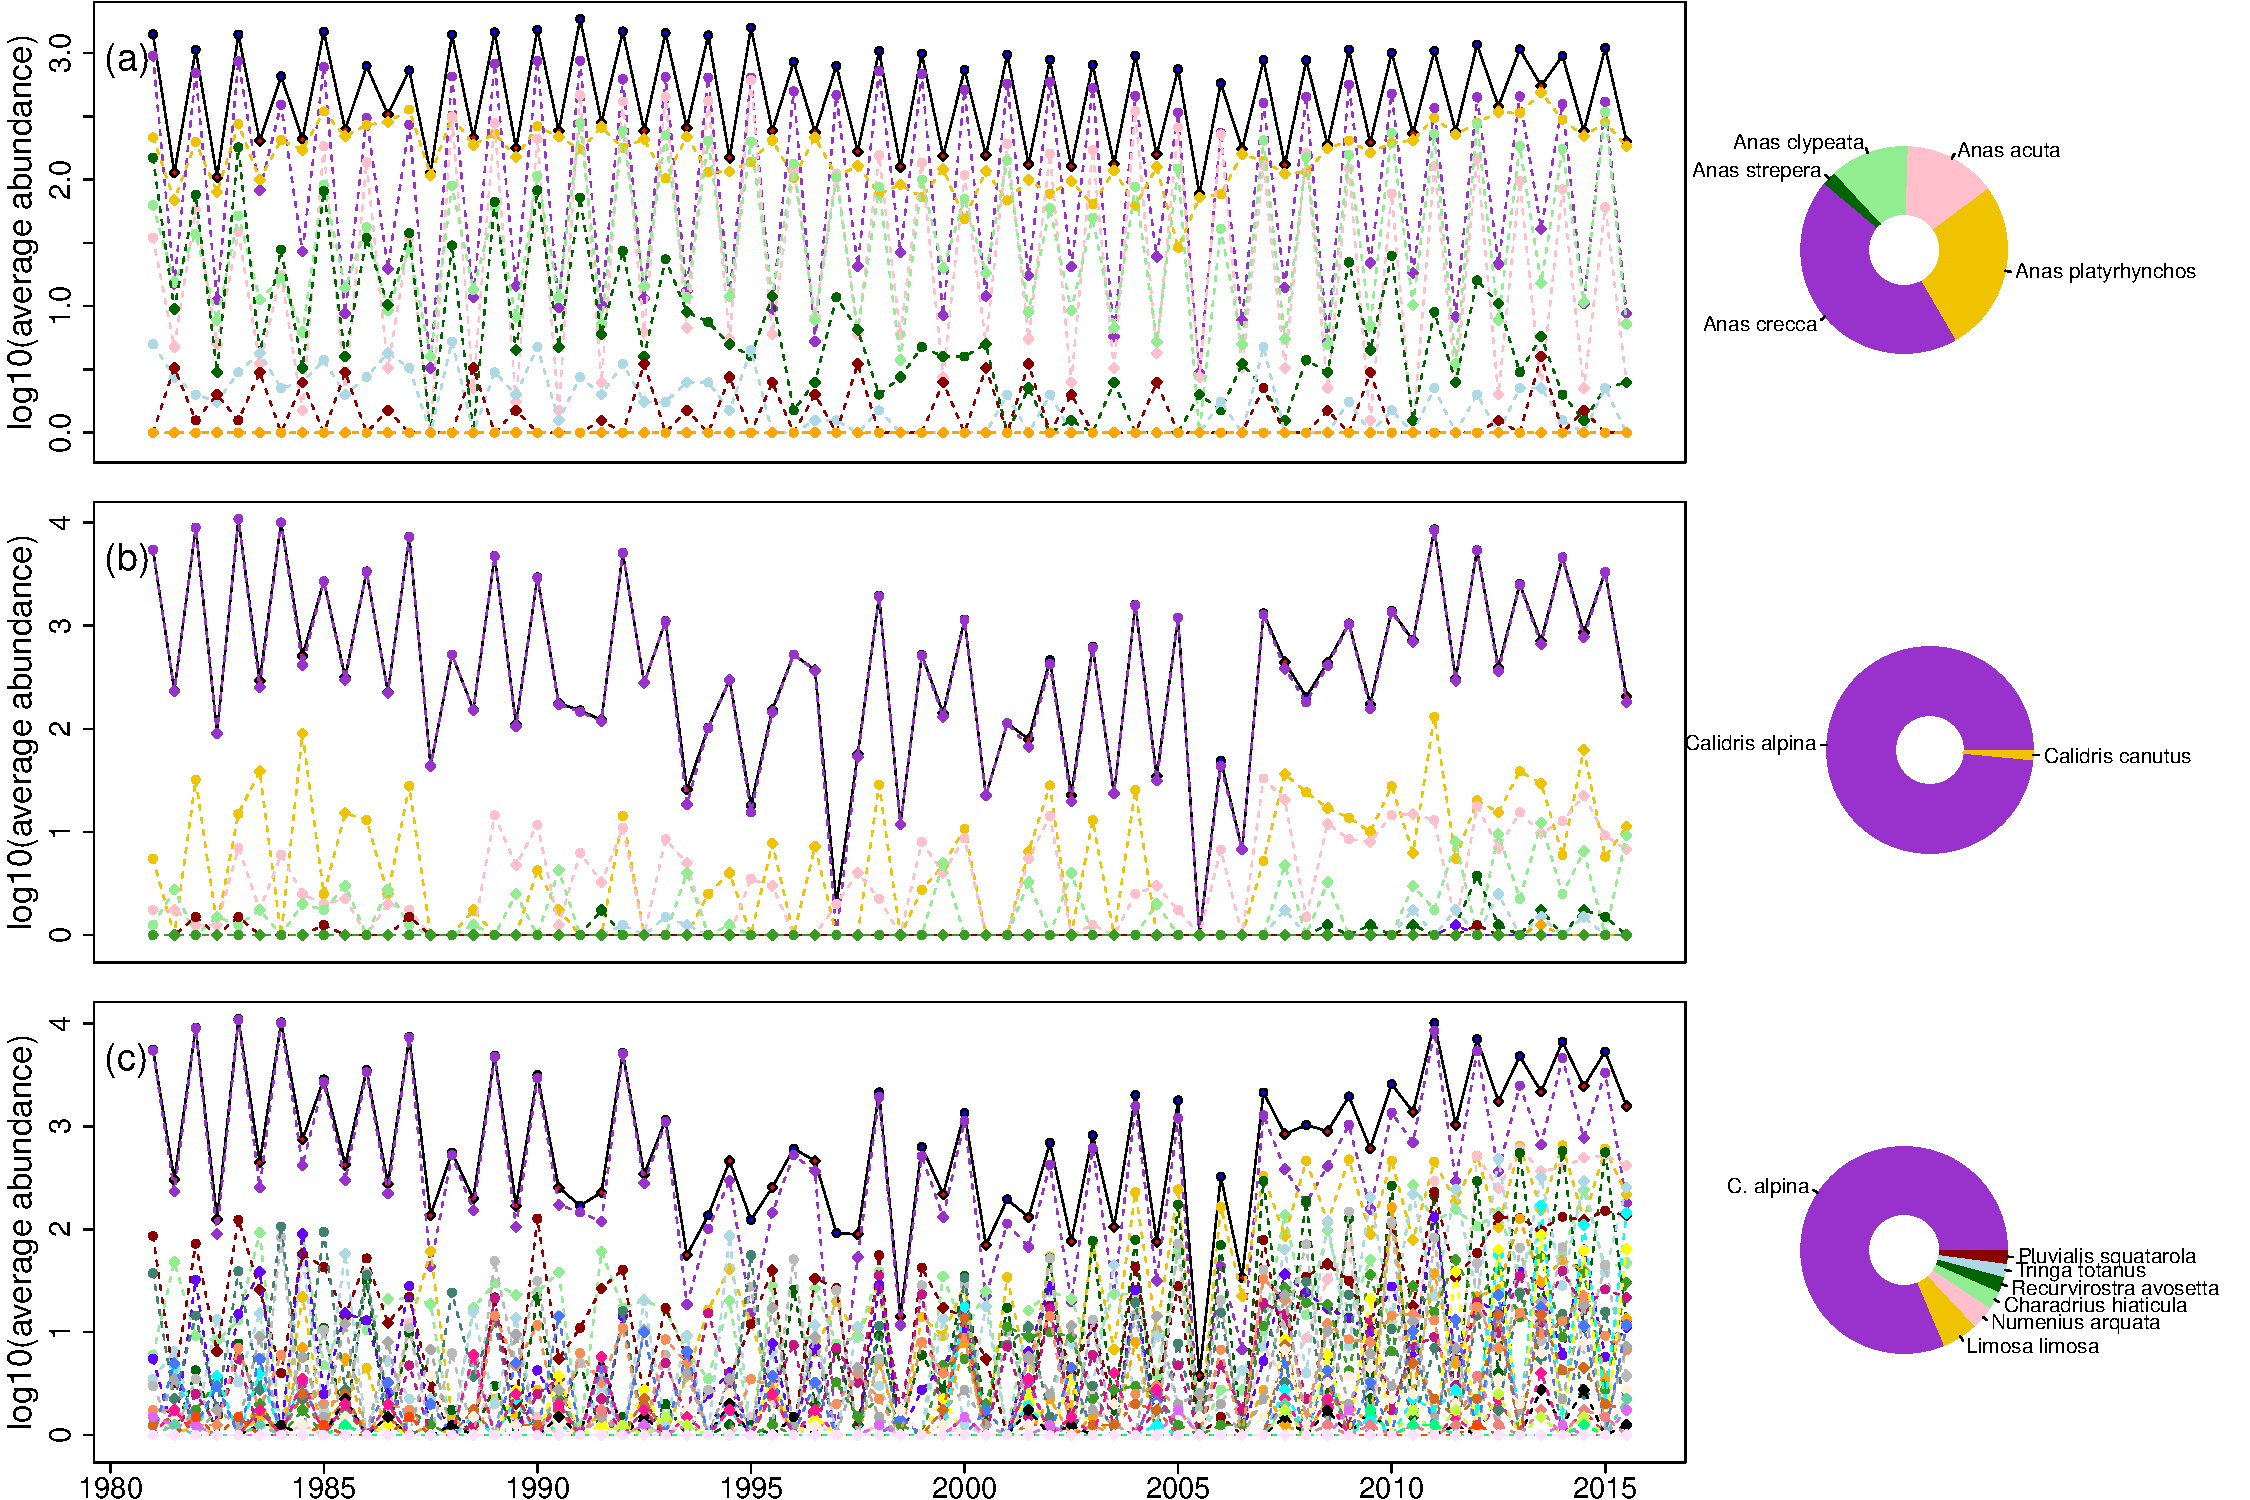
\includegraphics[width=18cm]{../OUT/average_abundance_timeseries}
\par\end{centering}
\caption{Time series of seasonally averaged abundance for\emph{ }ducks of the
genus\emph{ Anas} (a), calidrids (b, \emph{Calidris} genus), and all
waders (c, including calidrids). The solid black lines represent the
summed average abundances for each guild, dotted lines represent average
abundance for each species. Circles represent the cold season and
diamonds, the warm season. The coloured symbols below the curves represent
each species abundances, with species composition on the right side
on the donut plots for the most abundant species (over 1\% of relative
abundance in the group considered). \label{fig:Temporal-trends}}
\end{figure}


\subsection*{Statistical Analyses}

\subsubsection*{Yearly analyses}

We used for yearly analyses the synchrony index $\eta$ defined by
\citet{gross2013species}, which is constructed as the mean cross-correlation
between each species biomass and the summed biomasses of the rest
of the community (eq. \ref{eq:Gross}).

\begin{equation}
\text{\ensuremath{\eta}}=\frac{1}{n}\sum_{i}\text{Corr}(P_{i},\sum_{j\neq i}P_{j})\label{eq:Gross}
\end{equation}

where $P_{i}$ is the abundance or biomass of species $i$ in a community
of $n$ species. This synchrony index described in eq. \ref{eq:Gross}
varies between -1 (perfect compensation, total biomass is constant)
and 1 (complete synchrony), while 0 represents a case where all populations
fluctuate independently. Contrary to other indices (e.g., \citet{loreau_species_2008}'s
$\phi$), this index is independent from the richness $n$ of the
community (or more generally the number of system components) and
its overall stability \citep{bluthgen_land_2016,hallett_codyn_2016}.
This is particularly important here as we perform analyses at different
taxonomic scales, and therefore with a different $n$ in eq. \ref{eq:Gross}.

We computed synchrony indices at the year $\times$ season scale using
the codyn package in R \citep{hallett_codyn_2016}. That is, we constructed
two community-level time series where each year is associated to a
vector of species abundances, one for the cold season and one for
warm season. To do so, we averaged monthly bird abundances, for each
species, over the season duration. We then computed the synchrony
index for both cold and warm seasons using the year as our statistical
unit. In follow-up analyses, we also differentiated periods before
and after 2006, given that a management change occurred within the
reserve in 2006. We considered both the synchrony inside a given group
(e.g., among species of the \textit{Anas} genus) or between groups
(e.g., between the summed abundances of the 9 species of genus \textit{Anas}
and\emph{ }\textit{\emph{the sum of the 12 }}\textit{Calidris} species).
In the latter case of between-groups comparisons, we summed species
together before seasonal averaging, to consider seasonal averages
of the monthly group density.

We considered taxonomic classifications of the species (i.e., between
and within genera) and functional classifications of the species (e.g.,
30 species of waders vs 34 species of ducks) as we suspected that
a functional classification may allow to partition better the abiotic
requirements of the species. We use ``duck'' as a shorthand for
the larger functional group of herbivorous divers, because the birds
in that category are mostly ducks: this group includes nonetheless
all anatids (geese and swans in particular) as well as the common
coot \emph{(Fulica atra}, an abundant species here).

We also ``zoomed in'' on a group of species that were known to exhibit
potentially compensatory dynamics (through competition for roosting
sites): the great cormorant \textit{(Phalacrocorax carbo)}, the little
egret (\textit{Egretta garzetta}) and the grey heron (\textit{Ardea
cinerea}). The little egret and the grey heron abundances were summed
because of their similar requirements (i.e., they form a small functional
group).

We computed statistical significance of synchrony index values using
Monte Carlo randomizations \citep{gouhier_synchrony_2014}. For each
set of time series (each combination year $\times$ season), we kept
the auto-correlation of the species time series, but removed the cross-correlation
between species by shifting each time series by a random lag \citep{purves_fine-scale_2002}.
We obtained 100 sets of randomized time series for each season and
period of time considered and computed the corresponding synchrony
index. We then compared the observed values of $\eta$ to the values
obtained with the randomized time-series. Independence of species
was rejected at the Bonferroni-corrected 10\% threshold (a Bonferroni
correction is needed here because multiple comparisons across 2 seasons
and 3 periods). 

\subsubsection*{Wavelet analyses}

In addition to the time-domain analyses above, we performed frequency-domain
analyses for a range of temporal scales ranging from a few months
to years. This was done in particular for analyzing synchrony within
the rich wader community, as well as the group formed by the great
cormorant, grey heron and little egret.All wavelet analyses take as
input the monthly time series data.

Based on the work by \citet{keitt_coherent_2008} and follow-up by
\citet{vasseur_synchronous_2014}, we used the wavelet transform of
the time series to measure the coherency between time series

\begin{equation}
\rho(t,s)=\frac{\Lambda_{t,s}(|\sum_{k}w_{k}(\tau,s)|)}{\Lambda_{t,s}(\sum_{k}|w_{k}(\tau,s)|)}\label{eq:Keitt}
\end{equation}

where $w_{k}(\tau,s)$ is the continuous Morlet wavelet transform
of species $k$ at time $\tau$ for scale $s$, $\Lambda_{t,s}(\centerdot)=\int_{-\infty}^{+\infty}e^{-\frac{1}{2}(\frac{t-\tau}{s})^{2}}(\centerdot)d\tau$
and $|\centerdot|$ is the modulus of the complex number. The numerator
corresponds to the total biomass variation while the denominator corresponds
to the variations of each species. This index is close to 0 when species
compensate and reaches 1 when they are synchronous. As before, the
significance of each value was tested at the 10\%, Bonferroni-corrected,
threshold by 100 phase-randomizations of each species time series,
and computation of the corresponding $\rho$ values.

All datasets and statistical analyses are available in a GitHub repository
\url{https://github.com/fbarraquand/BirdTimeSeries_Teich}\footnote{Will be made public upon acceptance and archived in Zenodo}.

\section*{Results}

Using a taxonomic classification of the community (\textit{\emph{focusing
on the genera}} \textit{Calidris} and \textit{Anas} as two key examples
of contrasted birds), we can see that within-genus synchrony indices
at the seasonal scale are always positive whenever significantly different
from the null hypothesis (no temporal correlation between species),
i.e. there is no compensation within a genus (Fig. \ref{fig:Gross-synchrony-index}).
This matches the patterns obtained within the entire wetland bird
community (Fig A1 in Appendix 1).

For the cold season, \textit{Calidris} and \textit{Anas} exhibit opposite
trends in synchrony in response to the management change in 2006.
However, for the warm season, the management change, which consisted
in lowering the water levels, created more synchronous communities
of species within the \emph{Anas} and \emph{Calidris} genera. This
increase in synchrony after 2006 is matched by the functional group
classification.

Even though there is no widespread community-wide or genus-wide compensation
at the yearly timescale (differentiating the seasons), there could
be compensation at finer temporal scales, e.g. a month or two, or
coarser scales, over several years. When we consider the wavelet plot
(Fig. \ref{fig:Wavelet-modulus-ratio}), that is a time-varying and
scale-dependent strength of synchrony, we can see that there is synchrony
even at a fine temporal scale throughout most of the time series.
However, post-2006, there seems to be a possibility for overcompensation
on a scale around 5 years or around 3-4 months.

\begin{figure}[H]
\begin{centering}
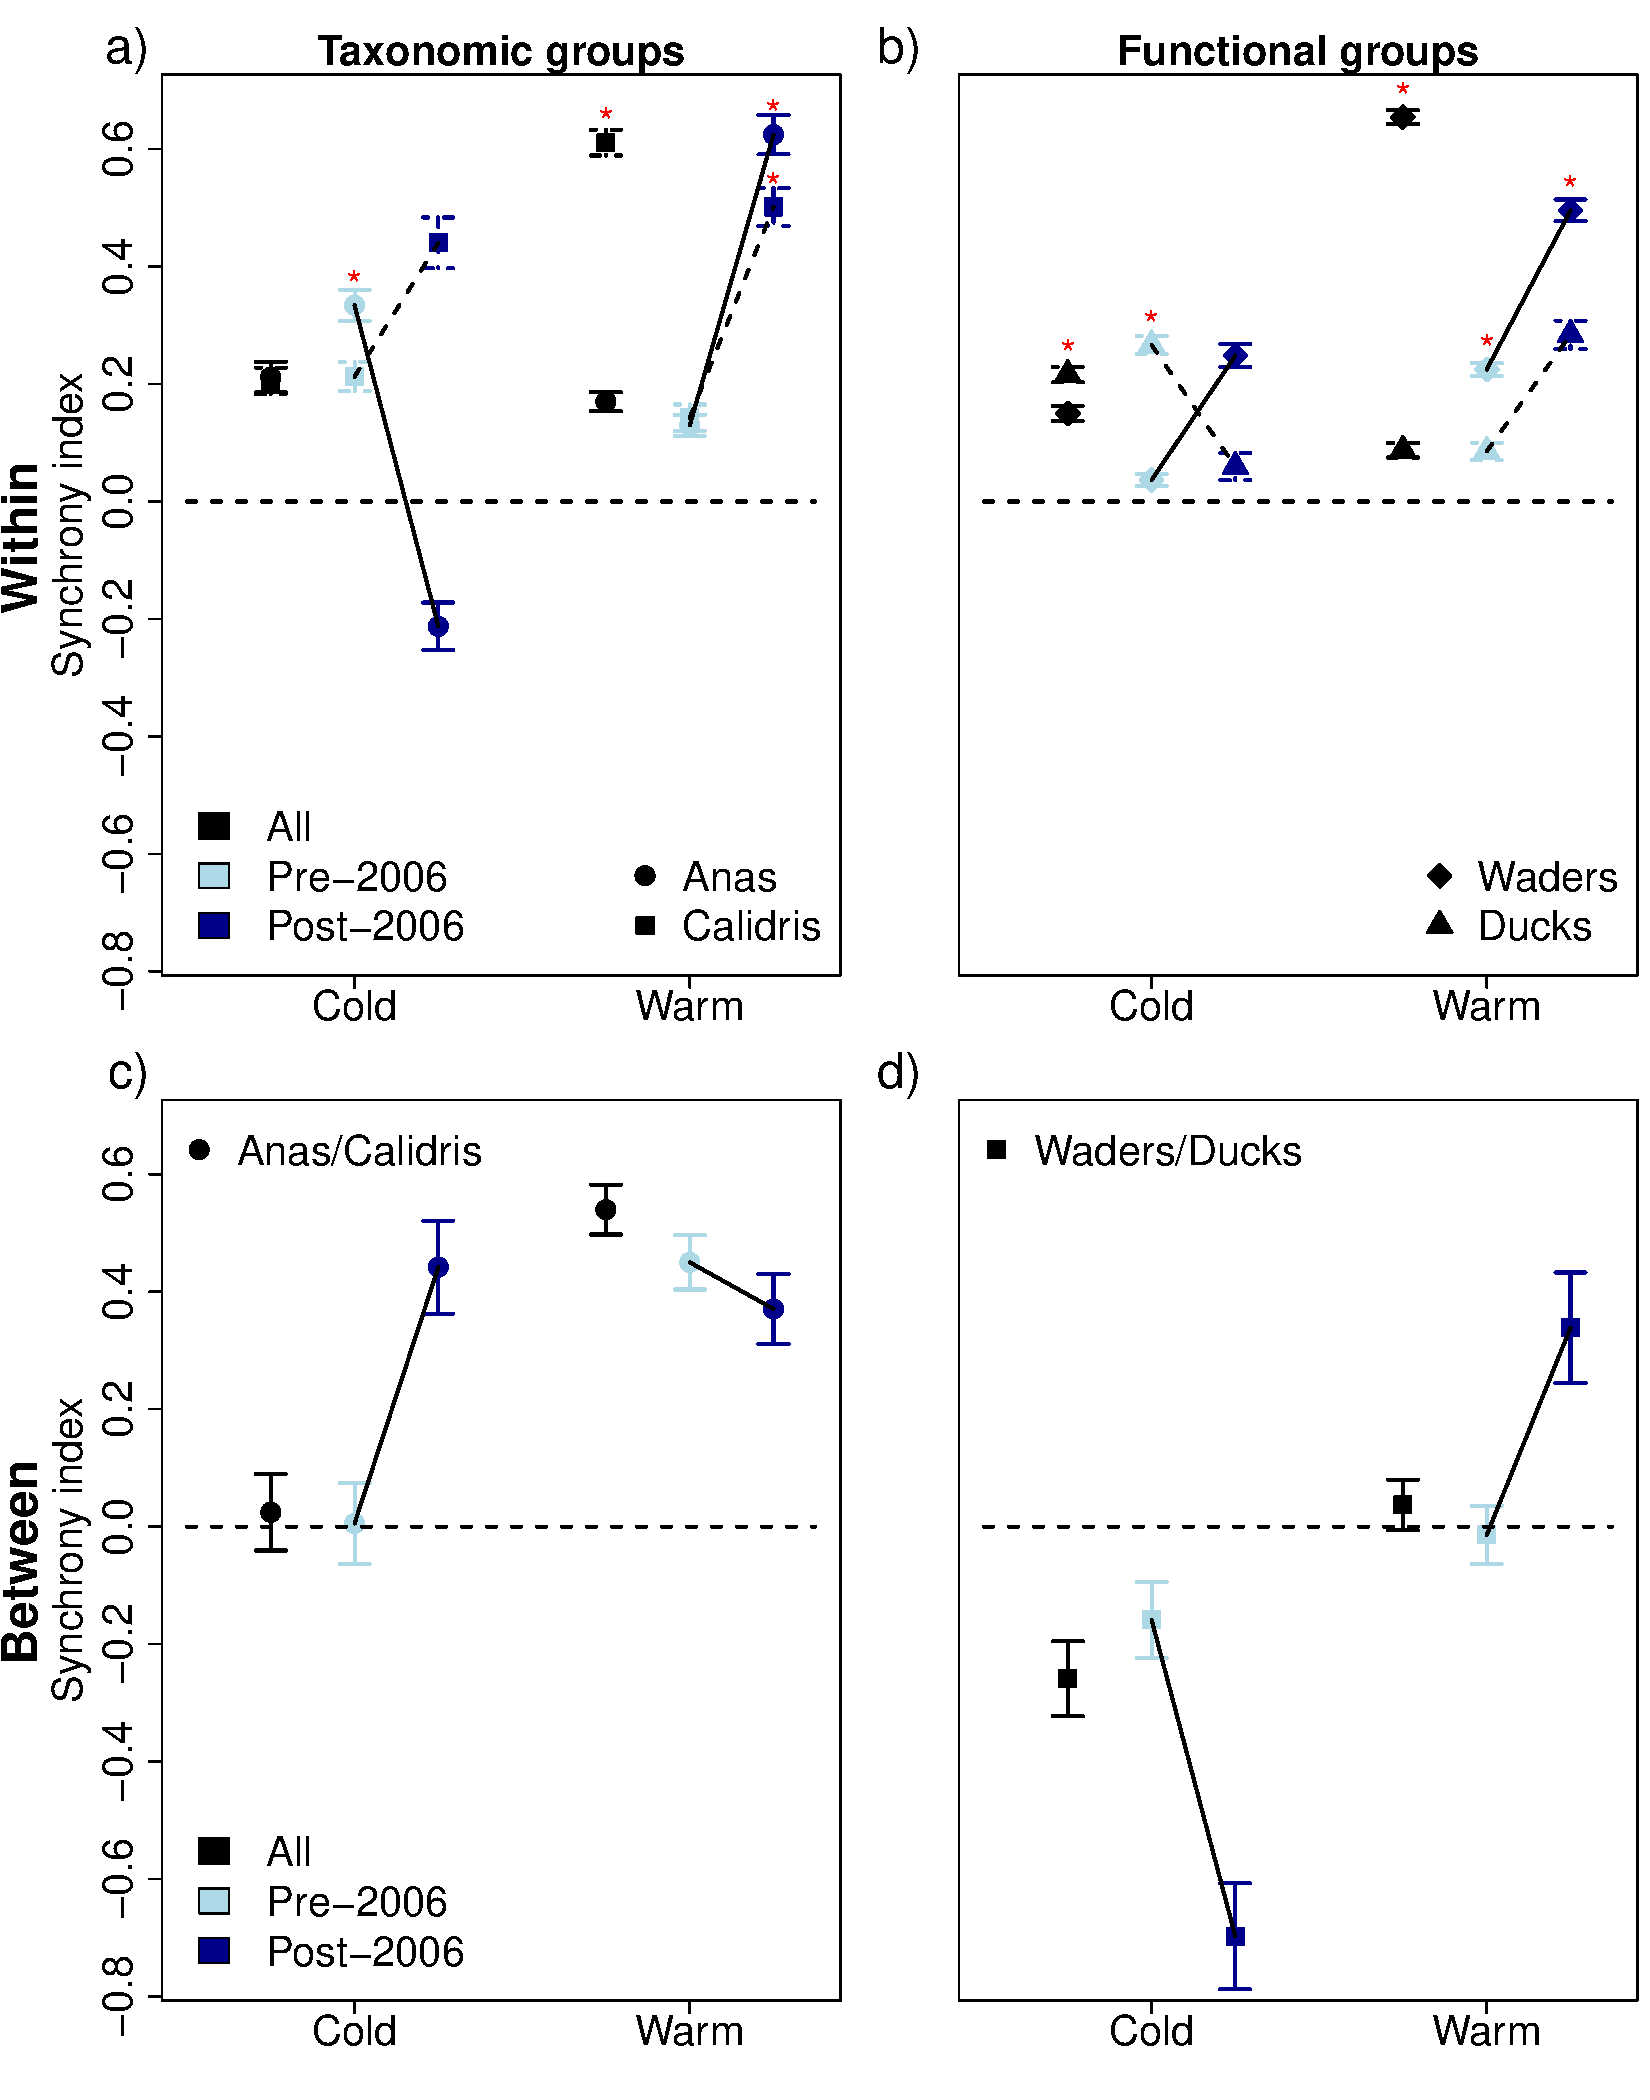
\includegraphics[width=0.85\textwidth]{../OUT/Fig2_new2_JAE}
\par\end{centering}
\caption{Gross' synchrony index ($\eta$) as a function of the season (cold
and warm seasons), calculated within (top, a-b) and between (bottom,
c-d) groups. The groups considered were different functional groups
(ducks vs waders, right b-d) or taxonomic groups (\emph{Anas} genus,
\emph{Calidris} genus, left a-b) groups. The index was computed in
each panel on the whole dataset (black) or using two periods: before
and after 2006 (light and dark blue), the year of the change in water
level management. Red stars correspond to synchrony values significantly
different from the null model (independent species), at the 10\% threshold.
\label{fig:Gross-synchrony-index}}
\end{figure}

There are therefore relatively contrasted results regarding the effect
of the management change on short-term synchrony within the wader
community. At the yearly (season) timescale, it seems to increase
the synchrony (though the Gross index and wavelets provide slightly
different answers). At even shorter timescales though, it seems to
decrease it.

More clear-cut results can be found when we examine the synchrony
vs compensation between functional groups (Fig. 2d). Since we consider
only two functional groups, the Gross index reduces to a simple correlation.
Waders and ducks are negatively correlated during the cold season
and positively correlated during the warm season. These patterns are
in contrast unclear when using a taxonomic classification (no compensation,
Fig. 2c). 
\begin{figure}[H]
\begin{centering}
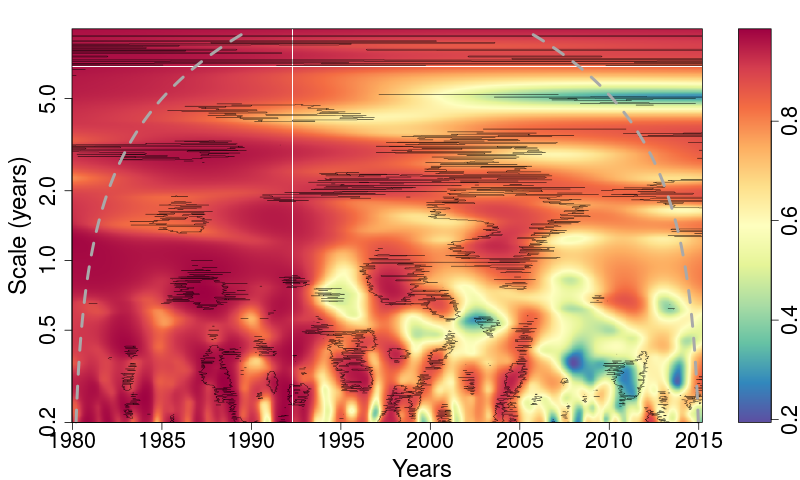
\includegraphics[width=0.95\textwidth]{Figure3} 
\par\end{centering}
\caption{Wavelet modulus ratio for the wader community, scaling from 0 (compensation,
blue color) to 1 (synchrony, red color). Dashed black lines delineate
regions significantly different from the null model (independently
fluctuating species) with a false discovery rate controlled at the
10\% threshold. \label{fig:Wavelet-modulus-ratio}}
\end{figure}

\begin{figure}[H]
\begin{centering}
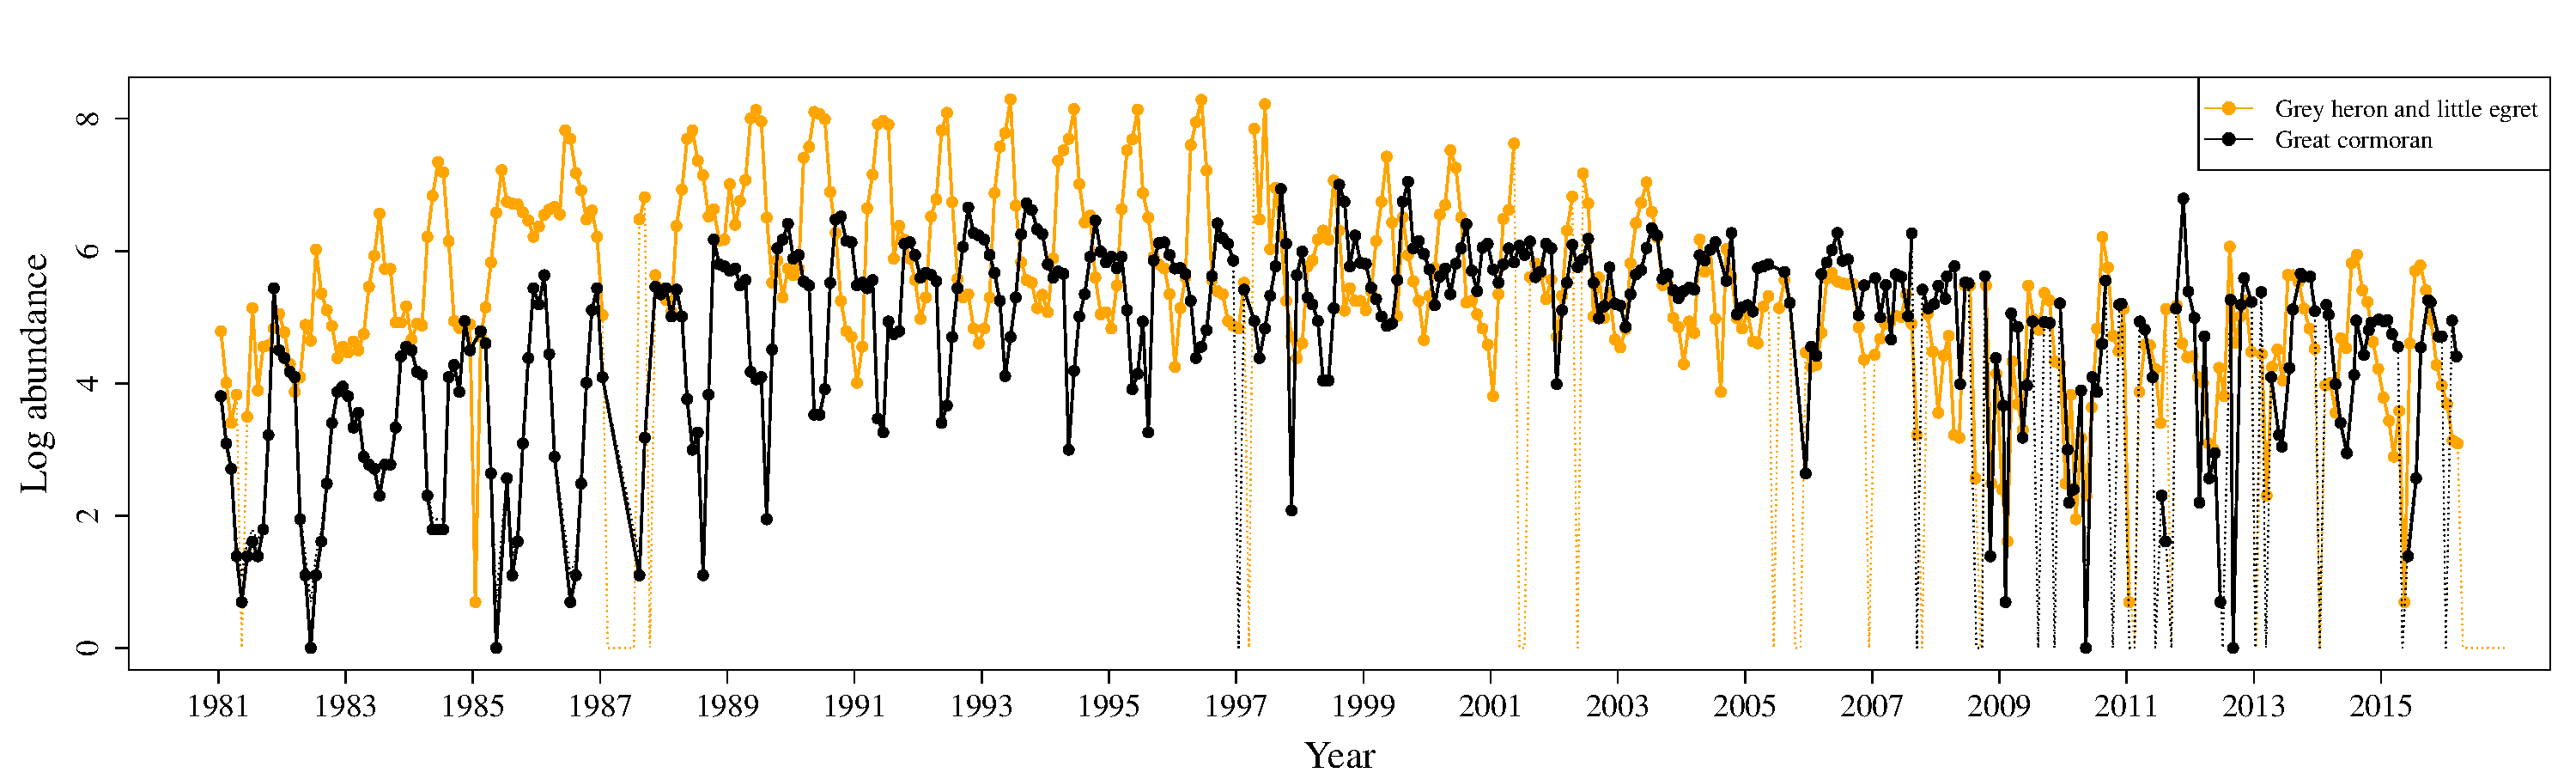
\includegraphics[width=1.1\textwidth]{Fig4} 
\par\end{centering}
\caption{Time series of great cormoran abundance, as well as summed abundances
of grey heron and little egret (logarithmic scale). \label{fig:Time-series-of}}
\end{figure}

\begin{figure}[H]
\begin{centering}
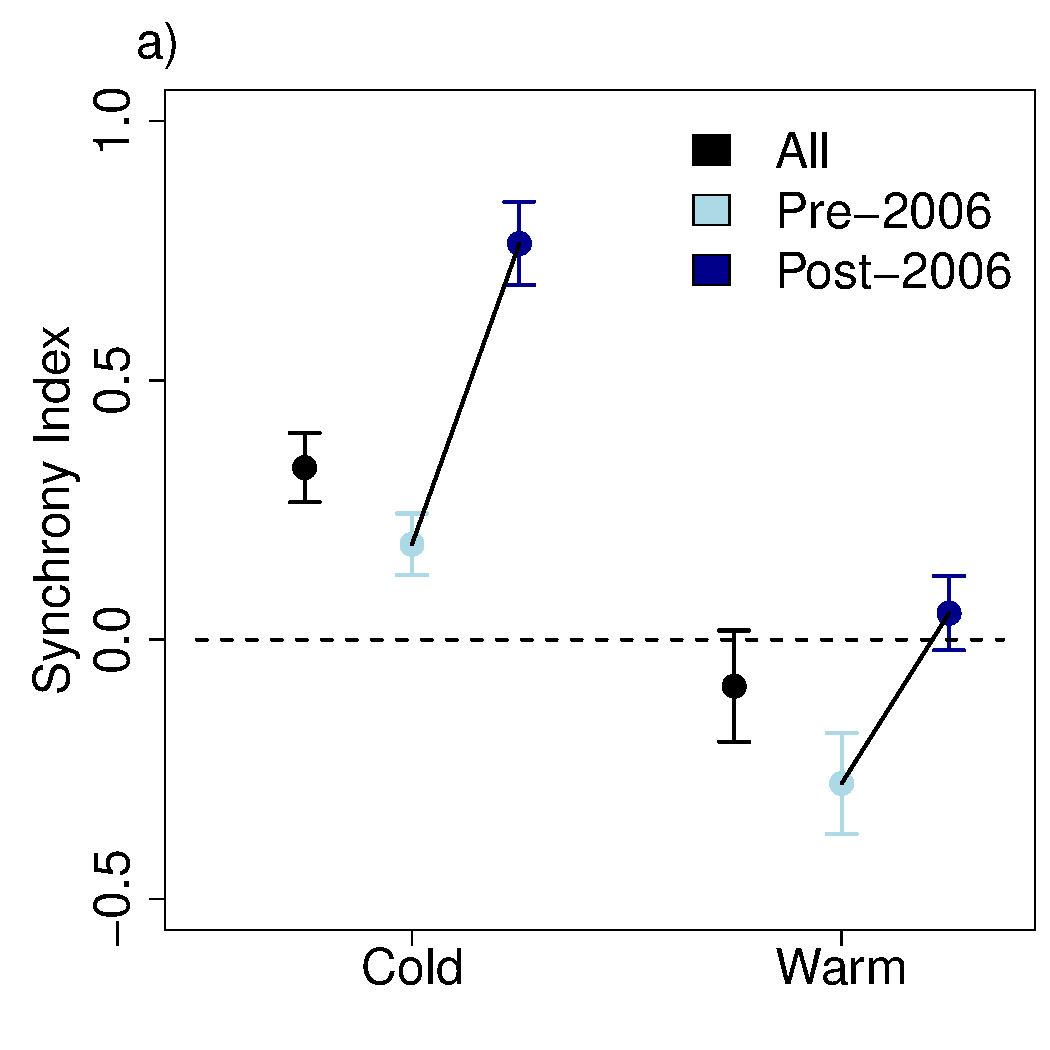
\includegraphics[width=0.55\textwidth]{../OUT/gross_triad_JAE}
\par\end{centering}
\begin{centering}
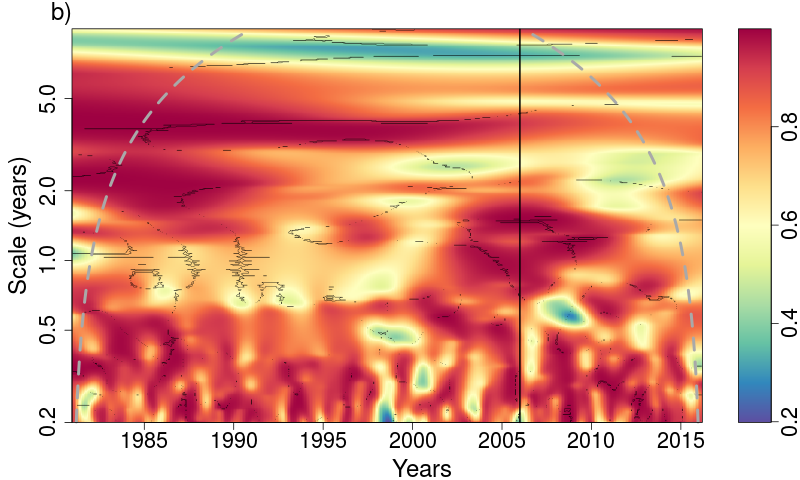
\includegraphics[width=0.7\textwidth]{wavelet_triad} 
\par\end{centering}
\caption{Time-domain (a) and frequency-domain (b) synchrony analyses of the
group formed by cormorant, egret and heron (see the captions of Fig.
\ref{fig:Gross-synchrony-index} and Fig. \ref{fig:Wavelet-modulus-ratio}
for symbol interpretation) \label{fig:Time-domain-(top)-and}}
\end{figure}

While compensation could be expected upon visual inspection of the
time series of the two groups formed by cormorant on the one hand,
and egret plus heron (summed as a small functional group) on the other
hand (Fig. \ref{fig:Time-series-of}), we see on Fig. \ref{fig:Time-domain-(top)-and}
that synchrony is in fact the rule around the annual scale and below,
when considering the wavelet index. We wondered if the patterns in
Fig. \ref{fig:Time-series-of} were caused by the use of a log scale,
but we found that in fact the correlation was higher rather than lower
on the log scale (Appendix 2). However, over long temporal scales
($\sim$ 6 years) there seems to be some compensation, which may indicate
a progressive change in composition within this small community module,
that was already visible on the time series plot (Fig. \ref{fig:Time-series-of}).
There might be some compensation over very short timescale as well
(within the season), but at very specific times and the biological
mechanisms for this are unclear, since these species compete for roost
sites, a process that it unlikely to manifest at such very short timescales.

\section*{Discussion}

Compensation was overall very rare at the yearly timescale (differentiating
between the cold and warm season). At short timescales (below the
season), and among taxonomically or functionally close species, some
compensation could be found but only at certain periods. In other
words, there was no widespread ``functional compensation'' (\textit{sensu}
\citealt{gonzalez2009causes}) \emph{within} genera or guilds at the
annual scale or below.

Yet, summing species abundances within a guild and comparing the ``biomass
sums'' of contrasted guilds, community composition did change in
frequency in the long run; in other words, there was some compensation
\emph{between} guilds.

Given that we compare the level of synchrony/compensation within guilds
(with many species) and between guilds (with only a handful of groups),
we checked in Appendix S4 if changing the number of ``compartments''
($n$) in the Gross $\eta$ index could affect its value: it did not.
However, we found that if two groups respond in opposite ways to a
shared driver, the stronger the response to the driver, the lesser
the compensation indicated by $\eta$ at the whole community level.
This might explain the low levels of compensation that we found at
the overall wetland bird community level (Appendix S2), in spite of
the clear presence of two groups reacting in opposite way to shared
driver (here, water levels). Analyses at several taxonomic/functional
scales are therefore warranted to be conclusive about compensation.

We used correlation between the summed abundances of closely related
species (species within the \textit{Anas} genus vs species within
the \textit{Calidris} genus) or the summed abundances of functionally
similar species (waders vs ducks) to uncover compensation. The functional
group classification produced much more clearly compensation between
guilds than the taxonomic classification. We expected to see compensation
at that ``functional scale'' irrespective of the season, because
the requirements of these birds are different, but here waders and
ducks were found to correlate negatively only during the cold (wintering)
season. This may be because the summer is characterized by a broad
inflow of birds, including non-resident individuals that somehow add
random variation to the community dynamics (though other explanations
are possible).

It may be better to say that we detected ``compensation'' rather
than ``compensatory dynamics'' between bird species \citep{gonzalez2009causes}
as the observed long-term changes in species composition (more waders,
proportionally less ducks; Appendix 4) might be due to an increased
inflow of birds preferring low water levels, and outflow of birds
preferring high water levels, under an overall space constraint. In
other words, the shift in community dynamics is likely not directly
due to birth and deaths. However, it would be incorrect to conclude
that such local compensation is disconnected from regional-scale community
dynamics: which species are present in the reserve affects their reproductive
success, which feeds back into regional-scale dynamics, and in turn,
regional-scale dynamics influences which species are locally settling
and competing.

Zooming in on the cormorant-heron-egret module, we find that compensation
mostly occurs above the annual temporal scale, and predominantly in
summer as well as before 2006. This occurs because of a slow replacement
of species due to competition for resting/roosting sites in the summer
season (C. Feign�, pers. obs.), which mostly occurred before 2006.

Overall, our results suggest to search for compensation more often\emph{
between} rather than \emph{within} functional groups, and over relatively
long timescales, above the typical temporal autocorrelation of the
dominant driver (e.g., above 5 years if the main driver is a seasonal
climate). This goes against calls to search for compensation at very
short timescales \citep{vasseur2007spectral,gonzalez2009causes},
below the timescale of the main synchronizing seasonal environmental
driver, in order to filter out its synchronizing effect. Although
searching for compensation at temporal scales below the seasonal abiotic
driver (e.g., temperature) was partly motivated by studies on plankton
whose community dynamics are much faster, with much shorter generation
times, we could have expected compensation to manifest also that scale
here as well (e.g., monthly). Indeed, movement of birds reacting to
food availability can certainly occur within the season, and wetlands
have a finite carrying capacity, so that there is competition for
space, which could promote short-term compensation. We suspect that
instead, because many species share common abiotic and biotic drivers
(e.g., disturbances due to nearby hunting) even below the yearly timescale,
their dynamics are bound to be synchronized to some degree even below
the yearly scale.

The attractor of community dynamics, i.e., the shape of community
trajectories in phase space, seems to be more or less an annual cycle
here: the dominant species fluctuate seasonally, but even though there
are shifts in some species dynamics, no abundant species seem to exhibit
violent multi-year oscillations. If we had to describe our community
mathematically, a dynamical model with a stable fixed point forced
by seasonality and some noise would probably work nicely. This mild
fluctuation scenario somehow constrasts with the dynamics of other
communities, such as insect pests, that have quite often multi-year
cycles (on top of seasonal cycles, for multivoltine species), with
possibly strong indirect interactions between similar species mediated
by predators and parasitoids \citep{murdoch2003consumer}. In this
latter context of internally-generated variability (\textquotedbl Endogenous
compensatory cycles\textquotedbl{} in \citealp{gonzalez2009causes}),
compensation is quite likely as well. \citet{klapwijk2018transient}
recently reported only transient synchrony between species of moths,
so that compensation could occur more frequently for more strongly
oscillating species. Therefore, compensation could be more likely
for those groups at the yearly timescale. Whether or not these findings
have some generality remains to be investigated by examining multi-species
synchrony for more varied animal taxa.

In many ways, searching for compensation using biodiversity time series
data is searching for needles in a haystack: only some specific temporal
and functional/taxonomic scales allow to see compensation whilst numerous
confounding factors make the community co-vary positively at all other
scales \citep{vasseur_synchronous_2014}. Although the knowledge of
specific biological mechanisms increasing the densities of some species
at the expense of others can help, synchrony will likely dominate
community-level time series data for closely related species, even
in species that compete strongly \citep{ranta_detecting_2008,loreau_species_2008}.
This is true even in cases of known mechanisms of competition for
space or shifts in community composition due to abiotic changes affecting
differentially species preferences, as in this study. We therefore
suggest that ``zooming out'' taxonomically or functionally (considering
summed abondances of dissimilar functional groups) and temporally
(considering temporal scales well above the periodicity of the dominant
abiotic driver) may often be the best strategy to see the compensation
that will inevitably manifest if the community-level biomass is to
be maintained within bounds.

\subsection*{Acknowledgements}

We thank the birdwatchers and staff of the Teich Reserve/Landes Gascogne
regional park who contributed to data collection over the years, as
well as LPO Aquitaine for helping us retrieve the raw data. The data
collection was supported by the Landes Gascogne regional park as well
as the Teich municipality, while data analysis was funded by LabEx
COTE (ANR-10-LABX-45). \\

\bibliographystyle{../Submission_Ecology/ecology}
\bibliography{BiblioTeich}

\end{document}
